% -*- mode:flyspell; mode:latex -*-
\documentclass[12pt]{article}

% \addtolength{\oddsidemargin} {-0.885in}
% \addtolength{\textwidth}{1.75in}
% \addtolength{\evensidemargin}{-0.8in}
% topmargin -0.5in
\usepackage[a4paper, top=1cm, left=1.5cm, right=1.5cm]{geometry} % width= , 

\usepackage[latin1]{inputenc}
\usepackage[T1]{fontenc}
\usepackage[english]{babel}
\usepackage{graphicx}
\usepackage{float}


\usepackage{tikz}
\usepackage{[caption}
\usetikzlibrary{arrows}
\usetikzlibrary{decorations.markings}
%\usepackage{lineno}

\usetikzlibrary{decorations.pathmorphing}
% \usepackage[absolute,overlay]{textpos}
% \usepackage{onimage}

\usepackage{times}
\usepackage{graphics}

% \usepackage{subfigure}
% \usepackage{scalefnt}
%
% \renewcommand\thesubfigure{\arabic{subfigure}}

\usepackage{amsmath}
\usepackage{hyperref}
\usepackage{hhline}
\usepackage{subfig}
\usepackage{color}
\usepackage[all]{hypcap}

\usepackage[normalem]{ulem}  % for striking out
% \usepackage{fancyhdr}
% \pagestyle{fancy}
% \fancyhead[C]{}
% \fancyhead[L] {\it{Mu2e-doc-29670-v1.0} }
%%%%%%%%%%%%%%%%%%%%%%%%%%%%%%%%%%%%%%%%%%%%%%%%%%%%%%%%%%%%%%%%%%%%%%%%%%%%%%
% use natbib - biblatex not available on Mu2e interactive nodes
%%%%%%%%%%%%%%%%%%%%%%%%%%%%%%%%%%%%%%%%%%%%%%%%%%%%%%%%%%%%%%%%%%%%%%%%%%%%%%
\usepackage[square,sort,comma,numbers]{natbib}

% location of the .bib files: env var BIBINPUTS (~/library/bibliography)

% \usepackage[backend=biber, style=numeric-comp, sorting=ynt] {biblatex}
% \addbibresource{clfv.bib}

% \addbibresource{stntuple.bib}
% \addbibresource{mu2e_web.bib}
% \addbibresource{radiative_pion_capture.bib}

\graphicspath{{figures/}}
%%%%%%%%%%%%%%%%%%%%%%%%%%%%%%%%%%%%%%%%%%%%%%%%%%%%%%%%%%%%%%%%%%%%%%%%%%%%%%
% for portability, make sure all commands are included locally
% order them alphabetically
%%%%%%%%%%%%%%%%%%%%%%%%%%%%%%%%%%%%%%%%%%%%%%%%%%%%%%%%%%%%%%%%%%%%%%%%%%%%%%
% \include{commands}

\newcommand {\keVc}       {\mbox{$\rm keV\!/\!c$}}
\newcommand {\kmax}       {\mbox{$k_{\rm max}$}}

\newcommand {\MeVc}       {\mbox{$\rm MeV\!/c$}}
\newcommand {\MeVcsq}     {\mbox{$\rm MeV\!/c^2$}}

\newcommand {\mumemconv}[1][A] {\mbox{$\mu^- \textrm{#1} \rightarrow e^- \textrm{#1}$}}
% Define a relay to have 2 default arguments instead of limit of 1
\newcommand {\mumepconv}[1][A] {%
  \def\ArgI{{#1}}%store the first argument
  \mumepconvRelay
}
\newcommand \mumepconvRelay[1][A]  {\mbox{$\mu^- \textrm{\ArgI} \rightarrow e^+ \textrm{#1}$}}
\newcommand {\muminus}    {\mbox{$\mu^-$}}
\newcommand {\muplus}    {\mbox{$\mu^+$}}
\newcommand {\MuToEm}     {\mbox{$\mu^- \ra e^-$}}
\newcommand {\MuToEp}     {\mbox{$\mu^- \ra e^+$}}
\newcommand {\MuPToEp}    {\mbox{$\mu^+ \ra e^+$}}
\newcommand {\ra}        {\rightarrow}
\newcommand {\tandip}    {\mbox{$\tan \lambda$}}

\newcommand {\Pb}[1]     {\mbox{$\rm ^{#1}Pb$}}                 % isotopes of lead
\newcommand {\Au}[1]     {\mbox{$\rm ^{#1}Au$}}                 % isotopes of gold
\newcommand {\Ir}[1]     {\mbox{$\rm ^{#1}Ir$}}                 % isotopes of iridium
%%%%%%%%%%%%%%%%%%%%%%%%%%%%%%%%%%%%%%%%%%%%%%%%%%%%%%%%%%%%%%%%%%%%%%%%%%%%%%
% editing commands
%%%%%%%%%%%%%%%%%%%%%%%%%%%%%%%%%%%%%%%%%%%%%%%%%%%%%%%%%%%%%%%%%%%%%%%%%%%%%%
\newcommand {\add}[1]    {{\red #1}}
\newcommand {\alt}[1]    {{\green #1}} %alternate comment color
\newcommand {\del}[1]    {{\blue \sout{#1}}}
\newcommand {\dlt}[1]    {{\violet \sout{#1}}} %alternate delete color

\newcommand {\black}     {\color{black}}
\newcommand {\red}       {\color{red}}
\newcommand {\blue}      {\color{blue}}
\newcommand {\strike}[1] {{\blue \sout{#1}}}
%%%%%%%%%%%%%%%%%%%%%%%%%%%%%%%%%%%%%%%%%%%%%%%%%%%%%%%%%%%%%%%%%%%%%%%%%%%%%%
\begin{document}

\begin{titlepage}
  \begin{flushright}
    \bf {MU2E/DAQ/47837} \\
    version 1.0
    \today
 \end{flushright}

  \vspace{1cm}

  \begin{center}
    {\Large \bf Commissioning of the tracker DAQ for the Vertical Slice Test

      \vspace{0.3in}

      1. Readout of a single ROC
    }

    \vspace{1cm}
    R.Bonventre (LBNL),
    S. Gamba  \footnote{\texttt{Fermilab; e-mail:s.gamba2\@studenti.unipi.it}} (University of Pisa),
    M.Tecchio (University of Michigan),
    P. Murat \footnote{\texttt{Fermilab; e-mail: murat\@fnal.gov}},
    V.Rusu  (FNAL)

        version 1.0
    \today
 \end{center}

  \begin{abstract}
    This note presents the initial results of the tracker DAQ commissioning performed in the fall of 2023.
    Readout of a single ROC connected to a DTC has been tested in several modes. A toy MC simulation
    of the ROC readout has been developed. The simulation results show a very good agreement with the data.
    \vspace{0.2in}
  \end{abstract}

\end{titlepage}
% \frontmatter
% \chapter*{Abstract}
%
% \addcontentsline{toc}{chapter}{Abstract}
%
% \mainmatter
%
{\tableofcontents}

%%%%%%%%%%%%%%%%%%%%%%%%%%%%%%%%%%%%%%%%%%%%%%%%%%%%%%%%%%%%%%%%%%%%%%%%%%%%%%%
%\chapter{Calibration}
%%%%%%%%%%%%%%%%%%%%%%%%%%%%%%%%%%%%%%%%%%%%%%%%%%%%%%%%%%%%%%%%%%%%%%%%%%%%%%%
% \input{input_data}

%%%%%%%%%%%%%%%%%%%%%%%%%%%%%%%%%%%%%%%%%%%%%%%%%%%%%%%%%%%%%%%%%%%%%%%%%%%%%%%
\newpage

\section {Notes for the authors}
\subsection {Revision history} 
\begin{itemize}
\item
  v1.01: initial version
\end{itemize}
%\linenumbers
\section {Introduction to the analysis}

In this note, we present initial results of the tracker DAQ commissioning.
\section{Description of teststand setup}
  The test stand included one DRAC card and one DTC connected to the DAQ computer,
  96 channels in total.
  The ROC was operated in the data readout mode, and the digi FPGAs were pulsed by the internal pulser.
  The pulser has two different frequencies,  31.29 MHz/(2$^7$+1), or approximately 250 kHz,
  and 31.29 MHz/(2$^9$+1), or approximately 60 kHz.
  The event window, that simulates the distance between proton pulses, could be varied by us.
  The ROC firmware has an internal hit buffer which can store up to 255 hits.
  That should be sufficient for the data taking.
  Testing therefore could proceed in two different modes:
  \begin{itemize}
  \item
    The event window is large enough , so the total number of generated hits is greater than 255. In this case
    the ROC hit buffer always gets filled up, and only the first 255 hits are read out;
  \item
    The total number of hits within the event window is less than 255.
    In this case the ROC hit buffer doesn't get filled up and the total number of hits
    can vary from one event to another.
  \end{itemize}

\begin{figure}[!h]
\centering
\includegraphics[width =0.8\textwidth]{figures/pdf/}
\caption{Graphic illustration of events.}
\label{fig:3}
\end{figure}
\section{Monte Carlo simulation}\label{MonteCarlo}

To ensure a comprehensive understanding of our system, we initiated a Monte Carlo Simulation of our Data Acquisition (DAQ) system. 
We simulated performances of the readout logic that is purely digital, relying on different assumptions.
Given that the maximum allowable number of hits per event is 255, the simulation follows these steps:
\begin{itemize}
  \item Within a time interval ranging from 0 $\mu$s to the reciprocal of the generator frequency, we generated the first event by following a uniform distribution;
    \item After verified that hits from the same channel, are separated by an interval equivalent to the reciprocal of the generator frequency, we proceeded to generate the second event by summing this specific time increment to the time of the first event;
      \item We verified whether the second pulse remained within the predefined event window. If it did, we included this hit in the ongoing event under construction;
      \item The process of event creation continued until the count of hits reached the maximum threshold of 255, at which point the event construction was terminated.
\end{itemize}
Furthermore, the simulation accounts for the channel to channel and FPGA to FPGA delays. 
This comprehensive approach ensures a faithful representation of the real-world operational aspects of the DAQ system.


%%% Local Variables:
%%% mode: latex
%%% TeX-master: t
%%% End:


%%%%%%%%%%%%%%%%%%%%%%%%%%%%%%%%%%%%%%%%%%%%%%%%%%%%%%%%%%%%%%%%%%%%%%%%%%%%%%
\section{Run 281: ``ROC buffer overflow'' mode}
%%%%%%%%%%%%%%%%%%%%%%%%%%%%%%%%%%%%%%%%%%%%%%%%%%%%%%%%%%%%%%%%%%%%%%%%%%%%%%
The readout configuration of Run 281 had the event window size of 50 us
and the pulser rate of 60 kHz

\subsection{Hit timing and occupancy}\label{over}
The first distributions to look at are the time distributions of hits in 
different channels and the distribution of the total number of hits
in a given channel (occupancy) as a function of the channel number.
The timing distributions of hits in channel 0 of the first FPGA
and in channel 2 of the second FPGA are shown in Fig.\ref{fig:1}.
The left distribution is, as expected, uniform, however the right one looks
less trivial.

\begin{figure}[H]
  \hspace{-0.5in}
  \begin{tikzpicture}
    \node[anchor=south west,inner sep=0] at (0,0.) {
      % \node[shift={(0 cm,0.cm)},inner sep=0,rotate={90}] at (0,0) {}
      % \makebox[\textwidth][c] {
      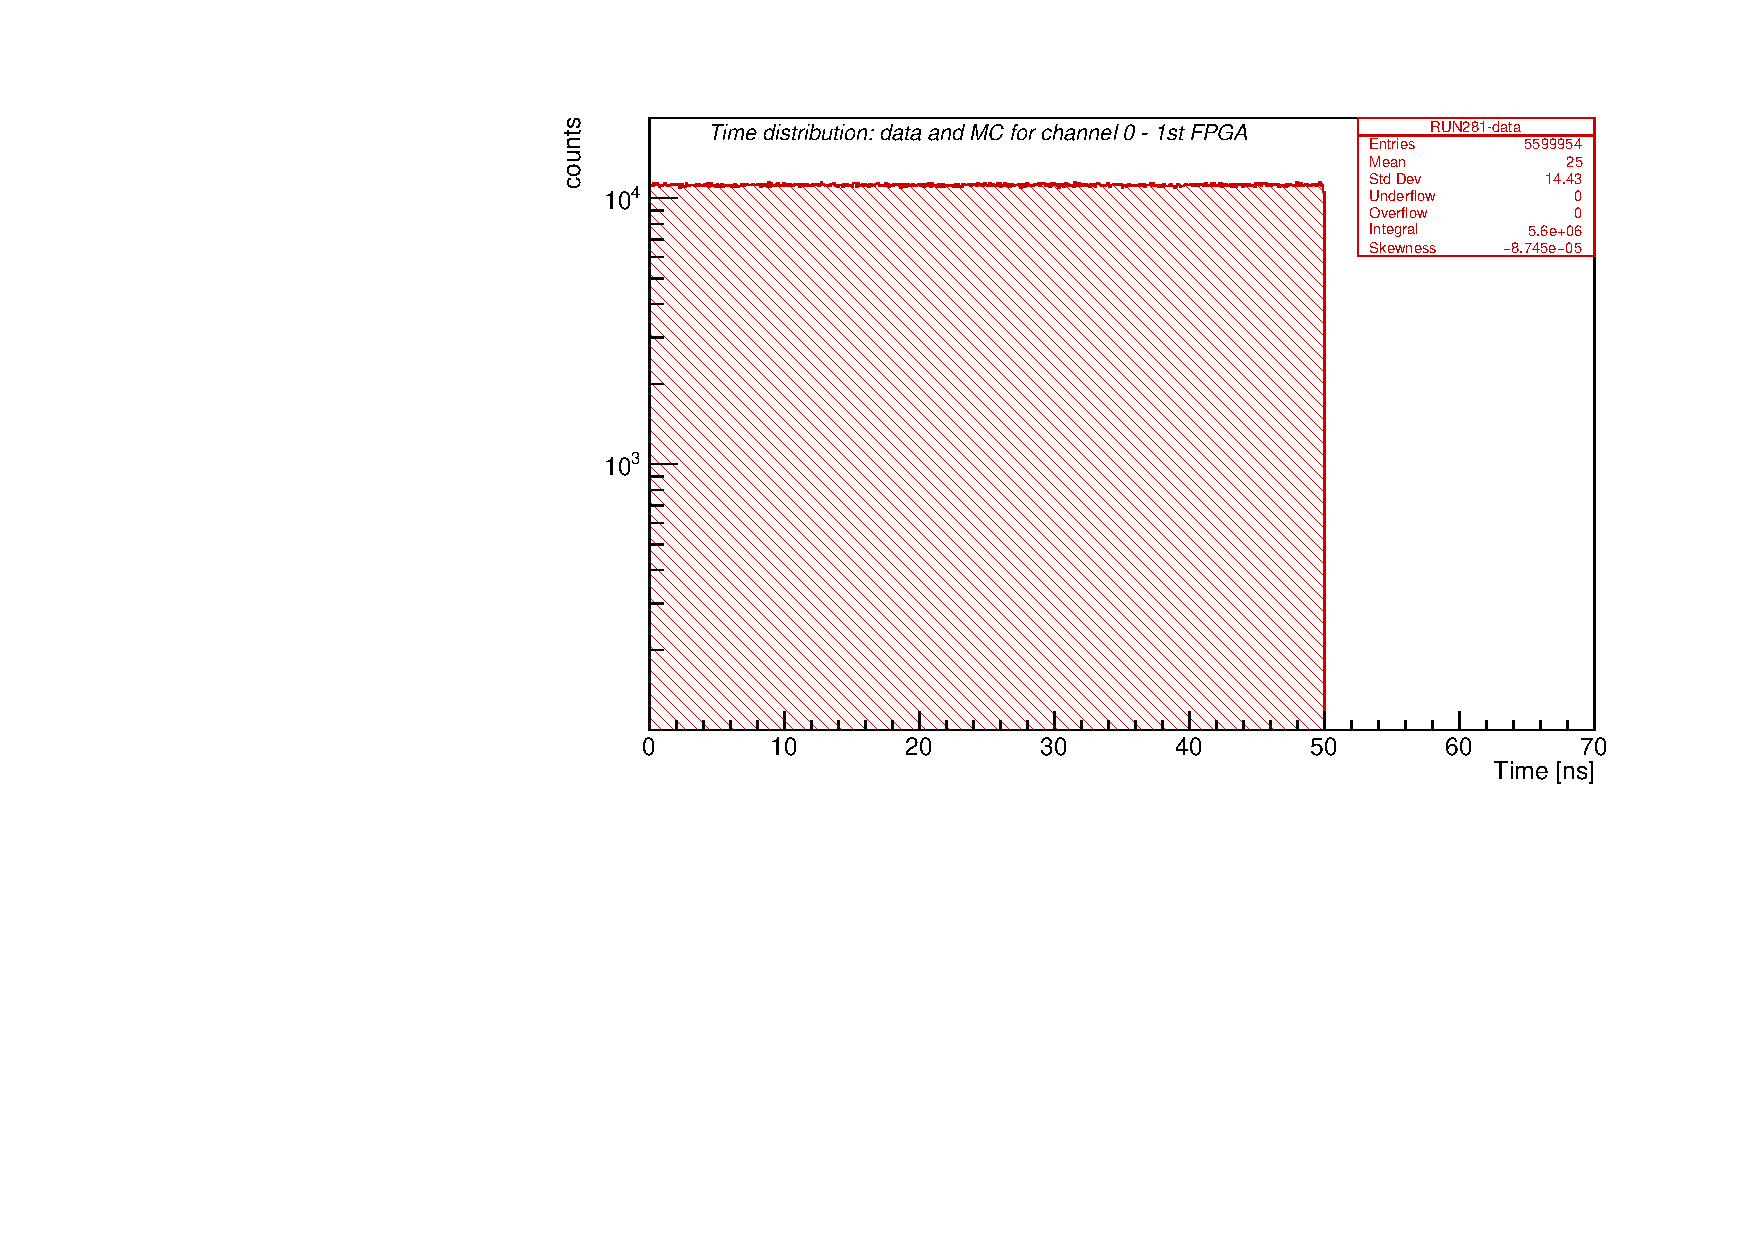
\includegraphics[width=0.5\textwidth]{figures/pdf/figure_00007_timedistr_roc_simulation_ch0_281}
      % }
    };
    \node[anchor=south west,inner sep=0] at (10,0.) {
      % \node[shift={(0 cm,0.cm)},inner sep=0,rotate={90}] at (0,0) {}
      % \makebox[\textwidth][c] {
      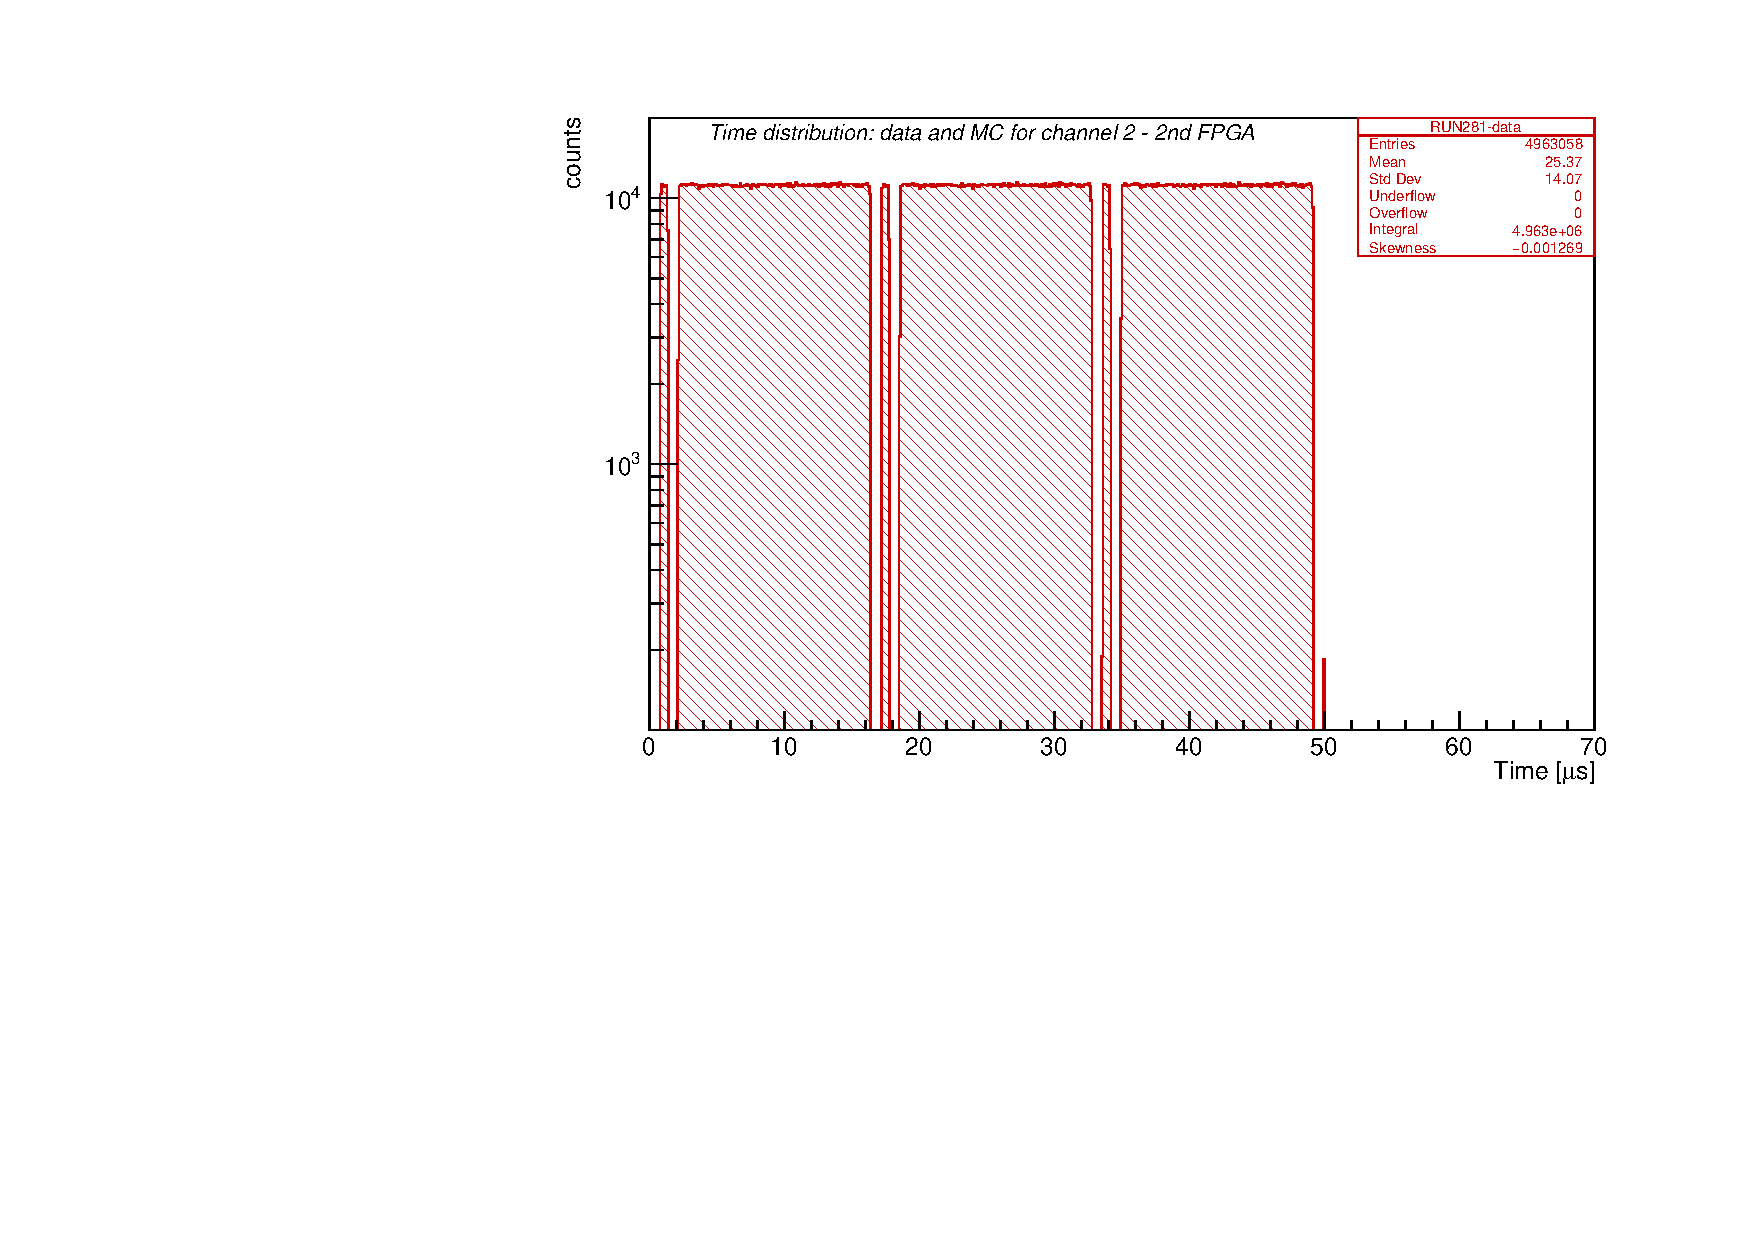
\includegraphics[width=0.5\textwidth]{figures/pdf/figure_00003_timedistr_roc_simulation_ch2_281}
      % }
    };
  \end{tikzpicture}
  \caption{
    \label{fig:1}
    left:
    time distribution of hits in the channel 0, first FPGA
    right:
    time distribution of hits in the channel 2, second FPGA
    }
\end{figure}

The distributions in Fig.\ref{fig:1} are easier to understand by looking at the occupancy plot in Fig.\ref{fig:2}.left.
The channel ordering in this plot corresponds to the readout order.
Channels in the beginning of the readout sequence always have all their hits read out,
  however that is not true for the channels in the end of the readout sequence.
\begin{figure}[H]
  \hspace{-0.5in}
  \begin{tikzpicture}
    \node[anchor=south west,inner sep=0] at (0,0.) {
      % \node[shift={(0 cm,0.cm)},inner sep=0,rotate={90}] at (0,0) {}
      % \makebox[\textwidth][c] {
      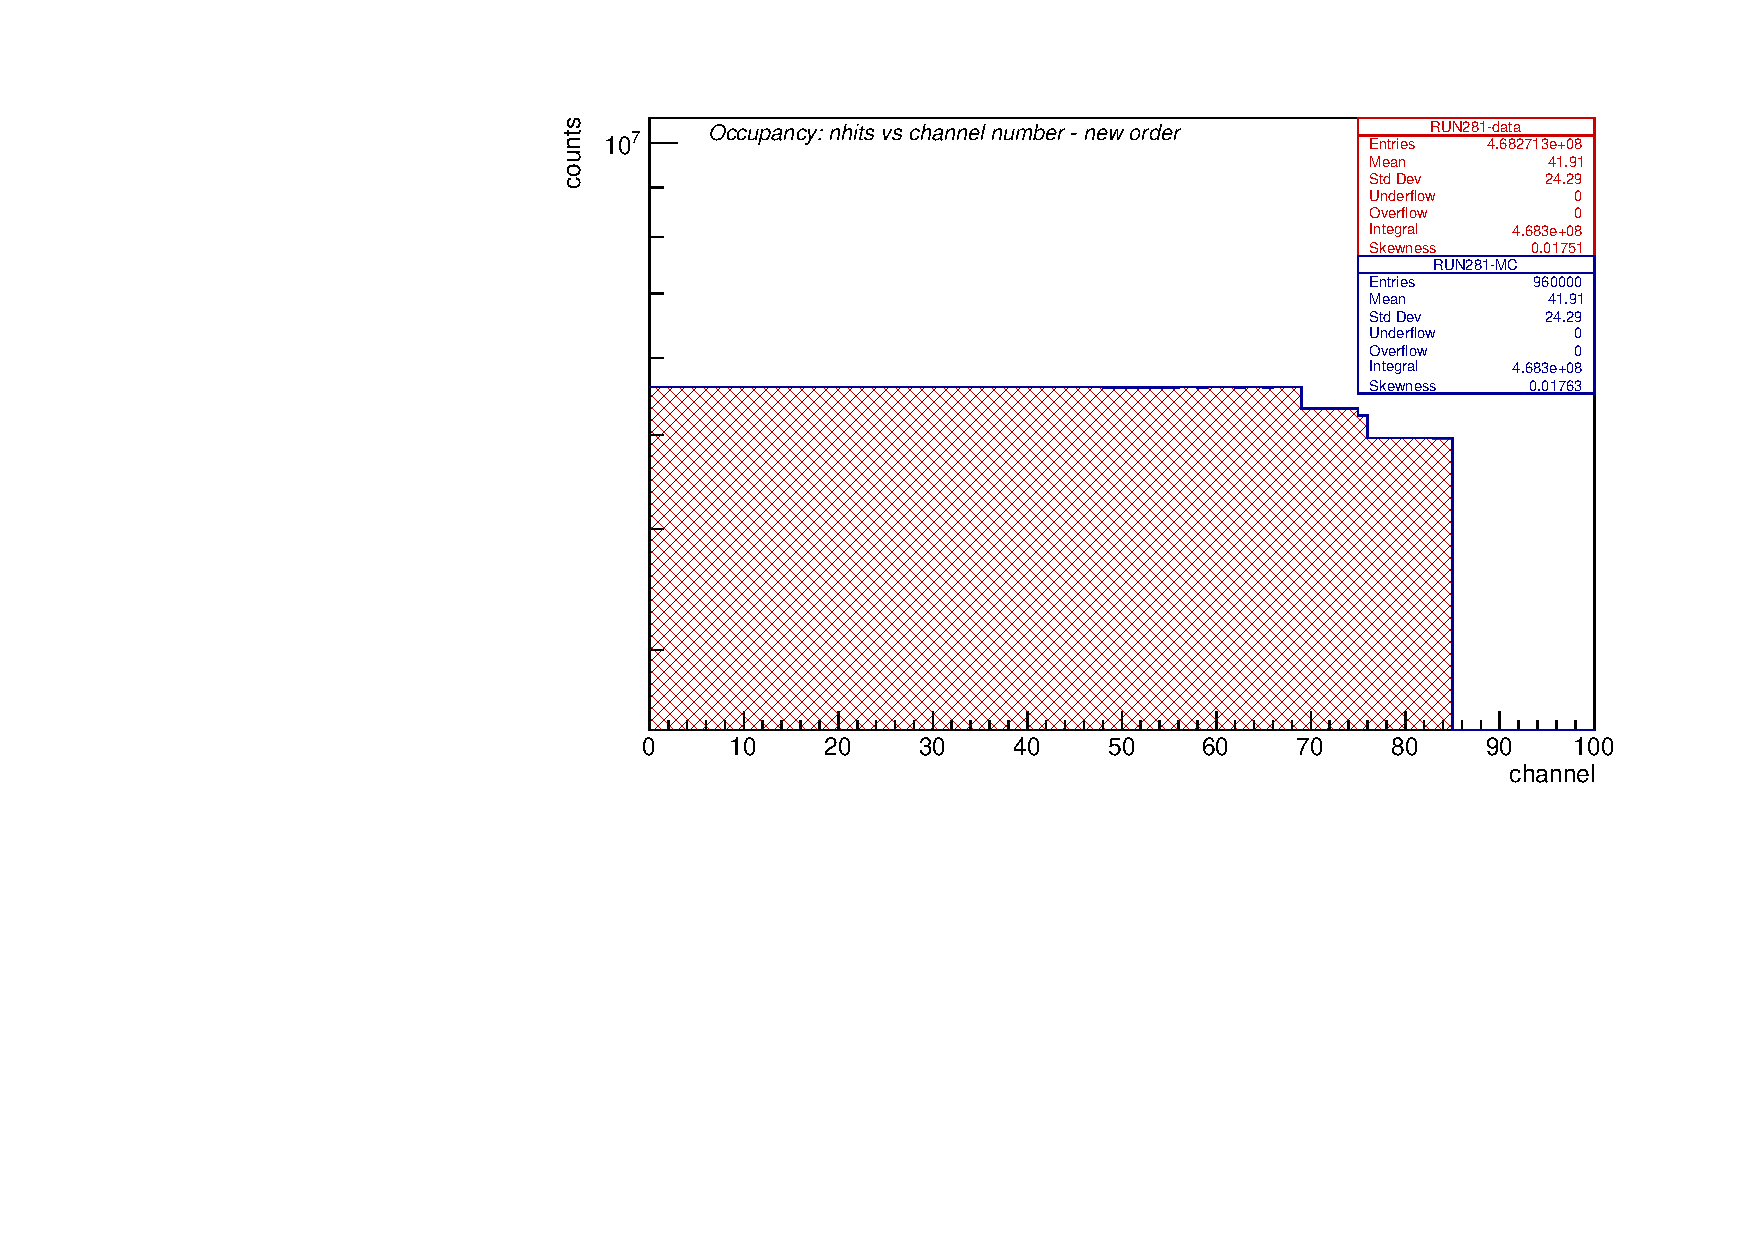
\includegraphics[width=0.5\textwidth]{figures/pdf/figure_00004_nhitsvschannel_roc_simulation_281}
      % }
    };
    \node[anchor=south west,inner sep=0] at (10,0.) {
      % \node[shift={(0 cm,0.cm)},inner sep=0,rotate={90}] at (0,0) {}
      % \makebox[\textwidth][c] {
      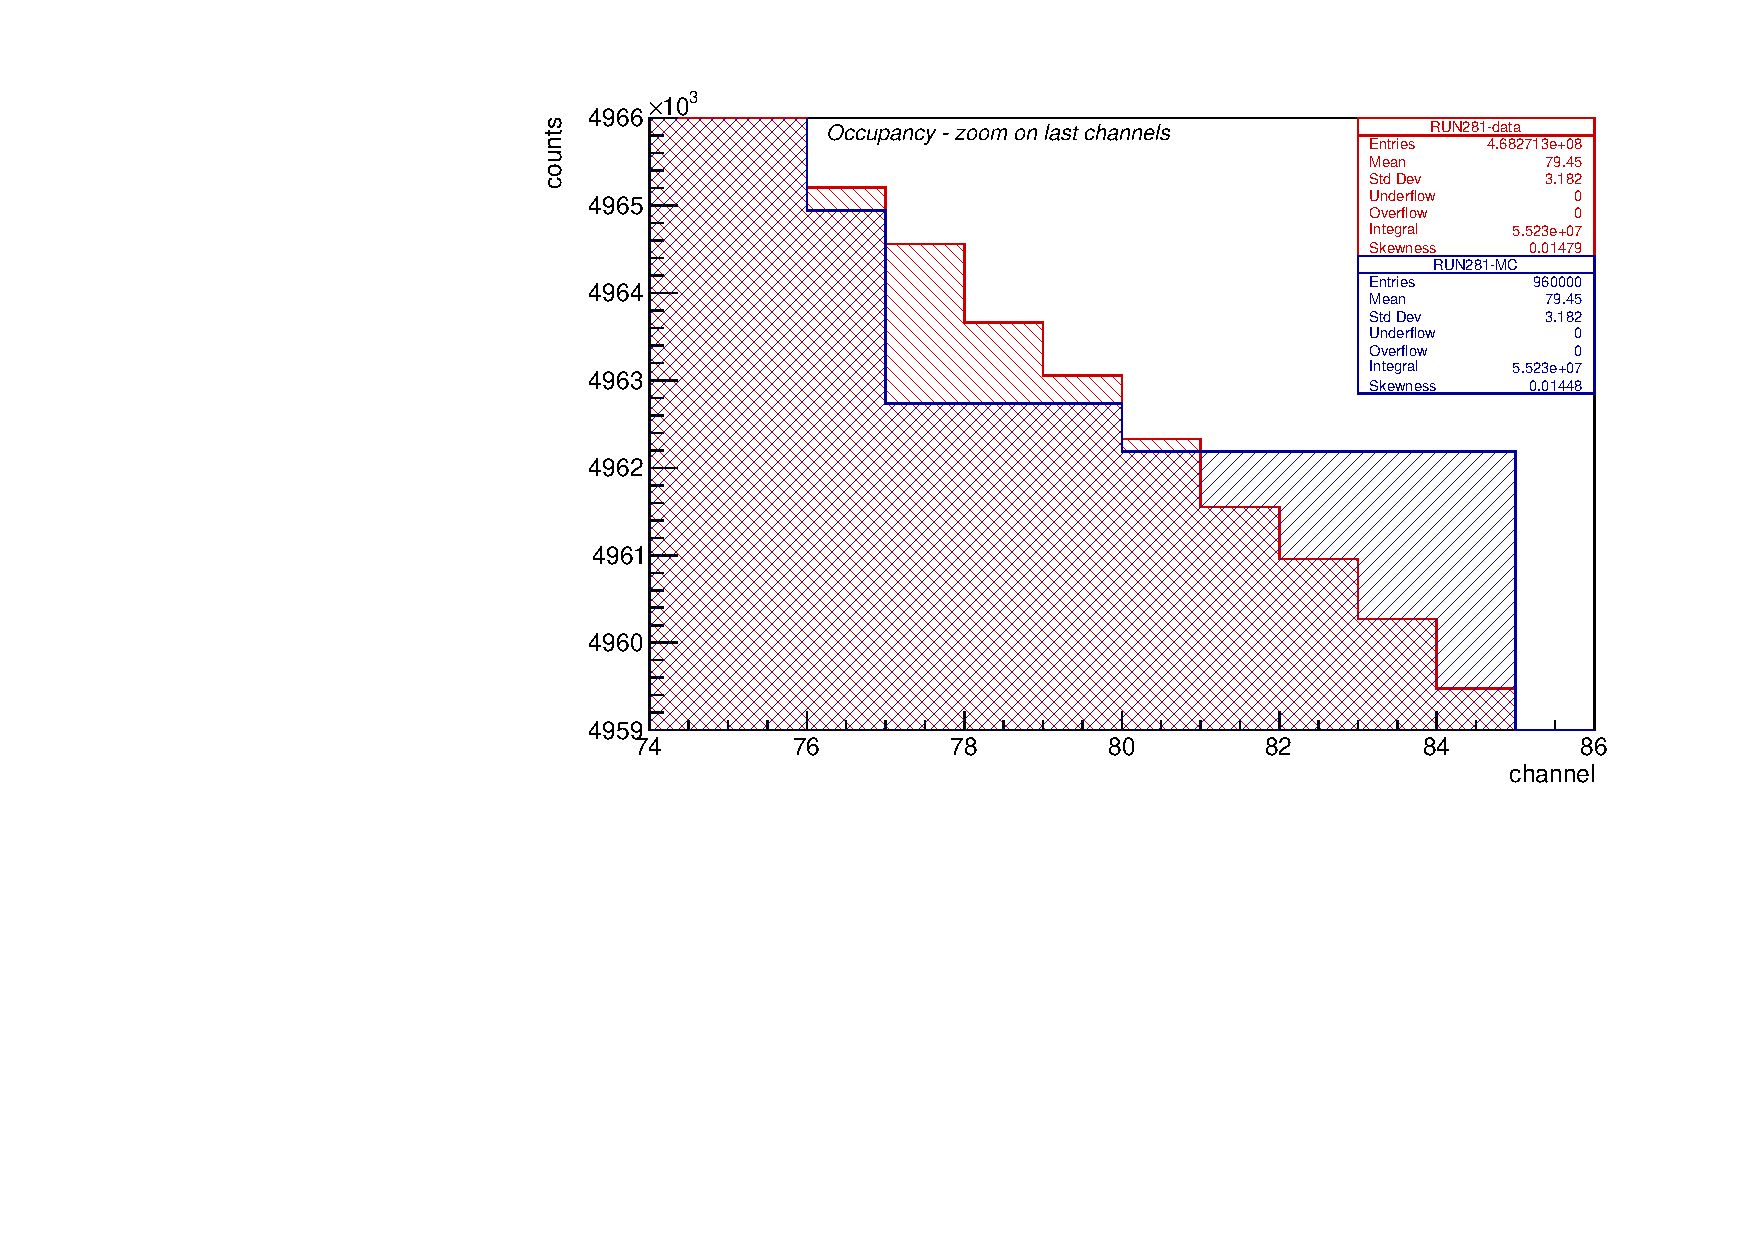
\includegraphics[width=0.5\textwidth]{figures/pdf/figure_00014_nhitsvschannel_roc_simulation_281}
      % }
    };
  \end{tikzpicture}
  \caption{
    \label{fig:2}
    left: number of hits versus the channel number.
    The channels are numbered in the readout order;
    right: zoom on the last channels in the readout sequence. The data and MC distributions
    differ from each other by $\sim$ 10$^{-3}$.
  }
\end{figure}

Figure \ref{fig:66} shows the distribution of the number of hits in channel 0.
For the event window of 50 us and the time between the pulses of 16 us,
the number of hits could be 3 or 4,
depending on the timing offset of a given readout window with respect to the generated timing sequence.
This distribution plays a key role in understanding of the occupancy plot.
\begin{figure}[H]
\centering
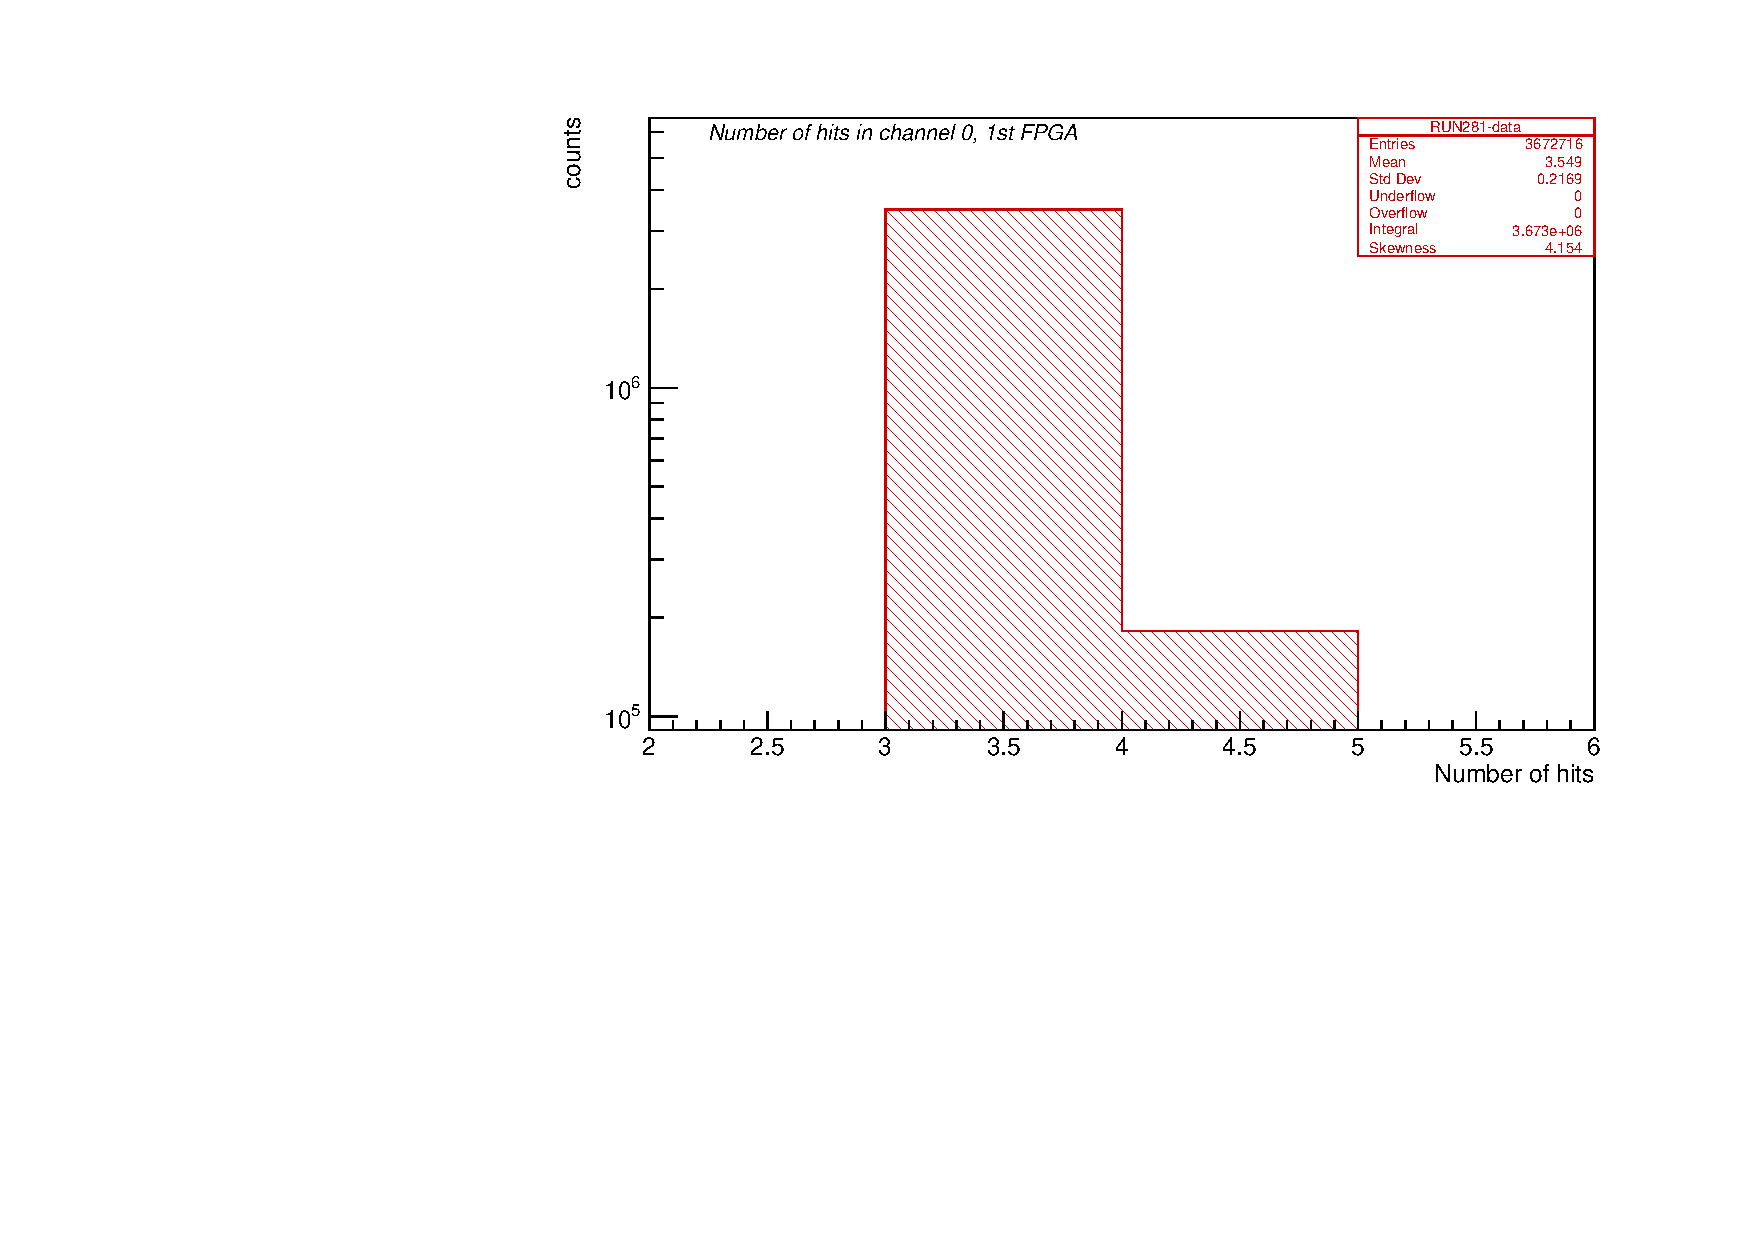
\includegraphics[width =0.8\textwidth]{figures/pdf/figure_00066_nhits_ch00_run281.pdf}
\caption{
  The distribution of the number of hits in the channel 0 of the first digi FPGA. for run 281
}
\label{fig:66}
\end{figure}

In the distribution shown in Figure \ref{fig:2}.left,
the first 68 channels are the ones with 4 hits per channel in the first FPGA
and three hits per channel in the second FPGA, 
resulting in the total of 255 hits.
The second plateau extending from 68 to 75 corresponds to the channels
with 3 hits per channel in the first FPGA and 4 hits per channel in the second one.
  The ``dent'' in the end of the second plateau is due to the fact that the 48 channels of the first FPGA
  yield 144 hits, so the second FPGA contributes 111 hits. The first 27 channels of the second FPGA contribute
  4 hits per channel each, but as 111 is not an integer of 4, the three hits from channel 28 in the readout sequence
  fill up the total ROC buffer of 255 hits.
There is a big step at the end of this plateau, because if we count the number of hits
in the first FPGA we get 144, so in the second FPGA we have 111 hits in total,
due to the fact that the maximum number of hits in total is 255.
111 is not divisible by 4, so the first 27 channels in the second FPGA will have 4 hits
and the last one will have 3 hits.
The last plateau corresponds to events with 3 hits per channel from the first FPGA
and 3 hits per channel from the second FPGA.

A zoom on last channels is shown on the right picture of Fig.\ref{fig:2}.
The relative difference between the data and the MC distributions is at a level of $10^{-3}$,
which is a very good agreement.
Coming back to Fig.\ref{fig:1}, the first channels in the readout sequence
always have all their hits read out,
while the channels in the end of the readout sequence - do not,
as the ROC hit buffer gets filled up after
the first 255 hits are read out.
This results in a uniform time distribution for the first channels readout and in a non-uniform
time distribution for the last readout channels, depending on $T_{gen}$ and $T_{EW}$.
The dips in the hit timing distribution for channel 2 are defined by the timing offset
between the two FPGA pulsers. 


%%%%%%%%%%%%%%%%%%%%%%%%%%%%%%%%%%%%%%%%%%%%%%%%%%%%%%%%%%%%%%%%%%%%%%%%%%%%%%
\subsection{Number of hits}
Fig. \ref{fig:3} shows that in the ``buffer overflow'' mode all events,
as expected, have 255 hits read out per event.

\begin{figure}[!h]
\centering
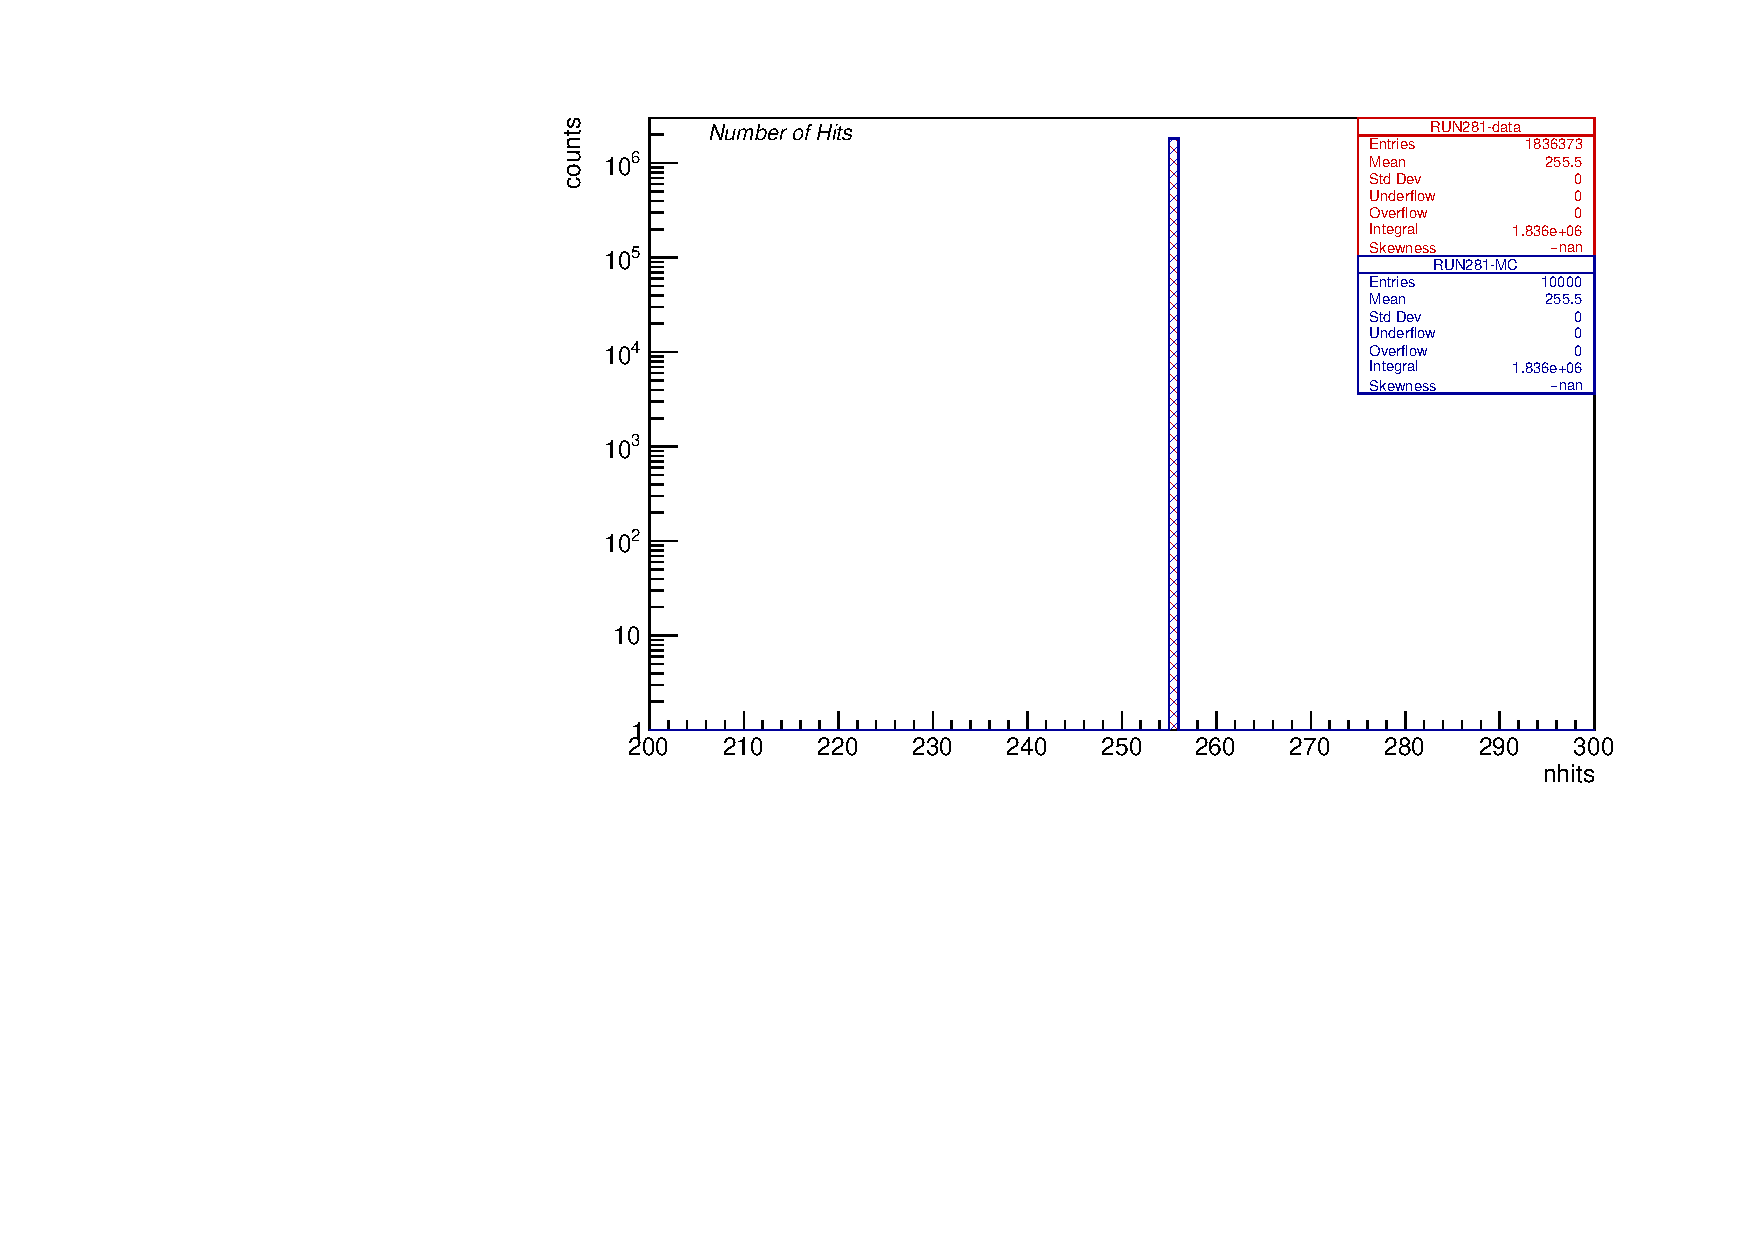
\includegraphics[width =0.8\textwidth]{figures/pdf/figure_00008_nhits_281}
\caption{
  The distribution of the total number of hits read out per event
}
\label{fig:3}
\end{figure}


%%% Local Variables:
%%% mode: latex
%%% TeX-master: t
%%% End:


%%%%%%%%%%%%%%%%%%%%%%%%%%%%%%%%%%%%%%%%%%%%%%%%%%%%%%%%%%%%%%%%%%%%%%%%%%%%%%
\section{Regular mode: RUN105038}
\subsection{Time distribution}
Similar to the approach outlined in Section \ref{over}, we commenced our analysis by investigating the temporal distribution of data for channels associated with the first and second FPGAs. Given that we are not operating in an overflow mode, our observations reveal a uniform temporal distribution for both cases.
\begin{figure}[H]
  \hspace{-0.5in}
  \begin{tikzpicture}
    \node[anchor=south west,inner sep=0] at (0,0.) {
      % \node[shift={(0 cm,0.cm)},inner sep=0,rotate={90}] at (0,0) {}
      % \makebox[\textwidth][c] {
      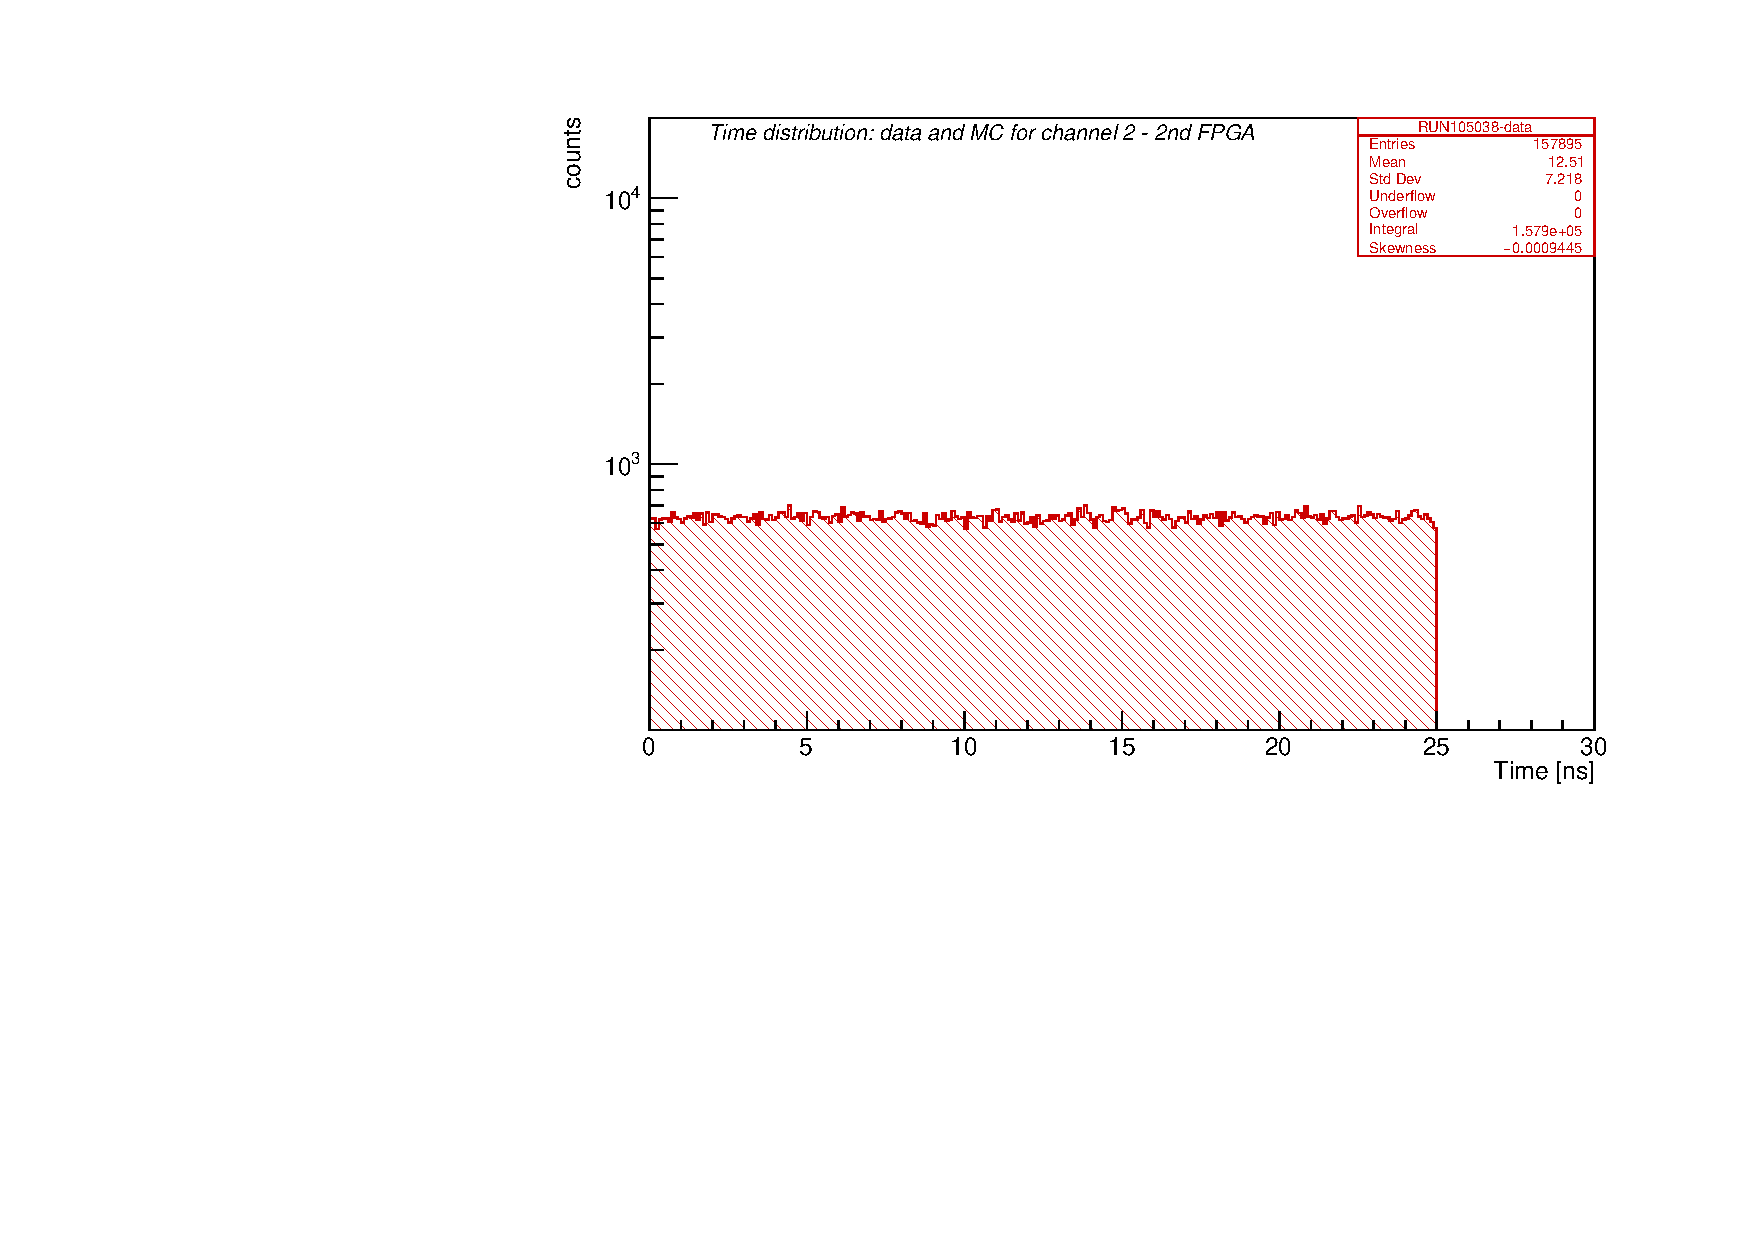
\includegraphics[width=0.5\textwidth]{figures/pdf/figure_00012_timedistr_roc_simulation_ch2_105038}
      % }
    };
    \node[anchor=south west,inner sep=0] at (10,0.) {
      % \node[shift={(0 cm,0.cm)},inner sep=0,rotate={90}] at (0,0) {}
      % \makebox[\textwidth][c] {
      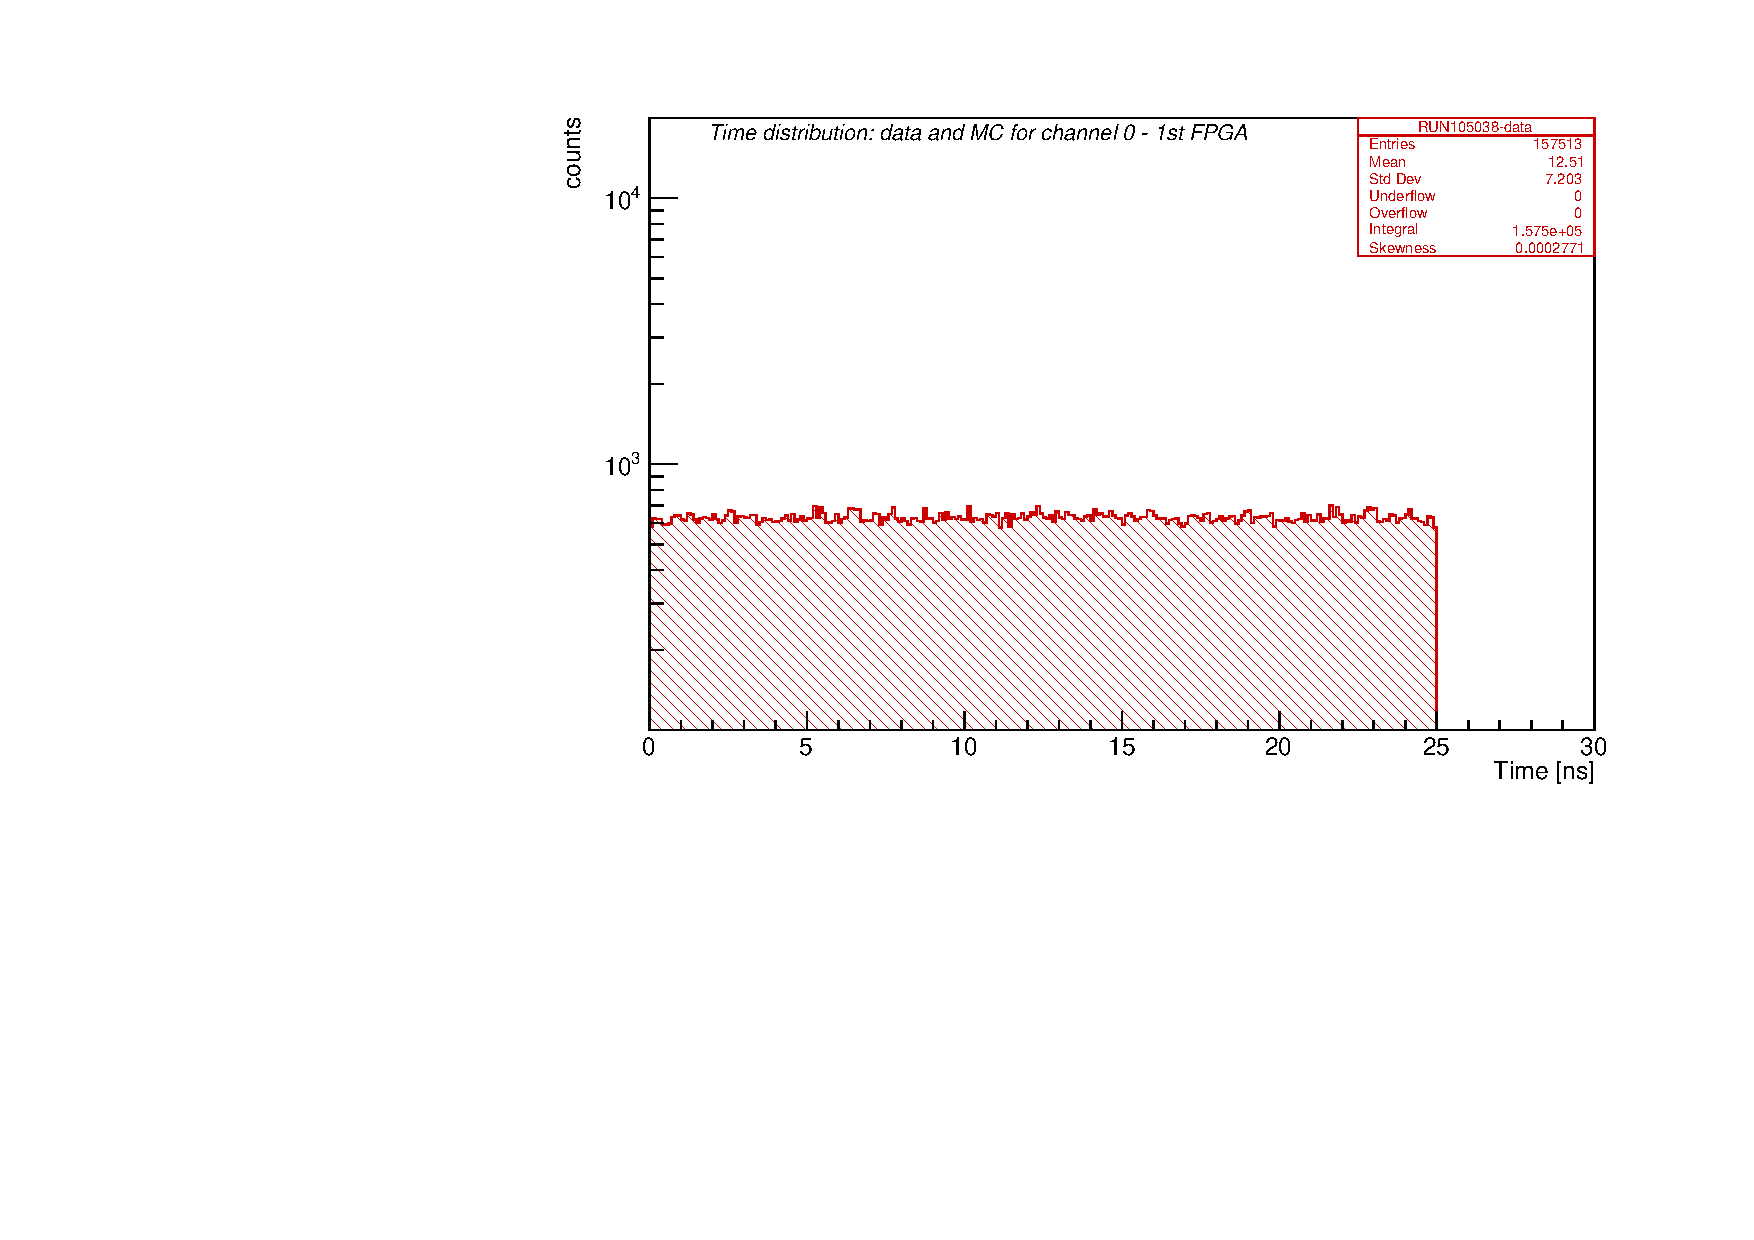
\includegraphics[width=0.5\textwidth]{figures/pdf/figure_00001_timedistr_roc_simulation_10538}
      % }
    };
  \end{tikzpicture}
  \caption{
    \label{fig:4}
    right: First FPGA's channel time distribution, left: Second FPGA's channel time distribution.
  }
\end{figure}
\subsection{Occupancy: Number of hits versus channel}
We conducted an analysis by reproducing the plot that shows the number of hits in relation to the channel number. The occupancy is a uniform distribution, primarily attributable to the fact that we are operating in a non-overflow mode.
\begin{figure}[!h]
\centering
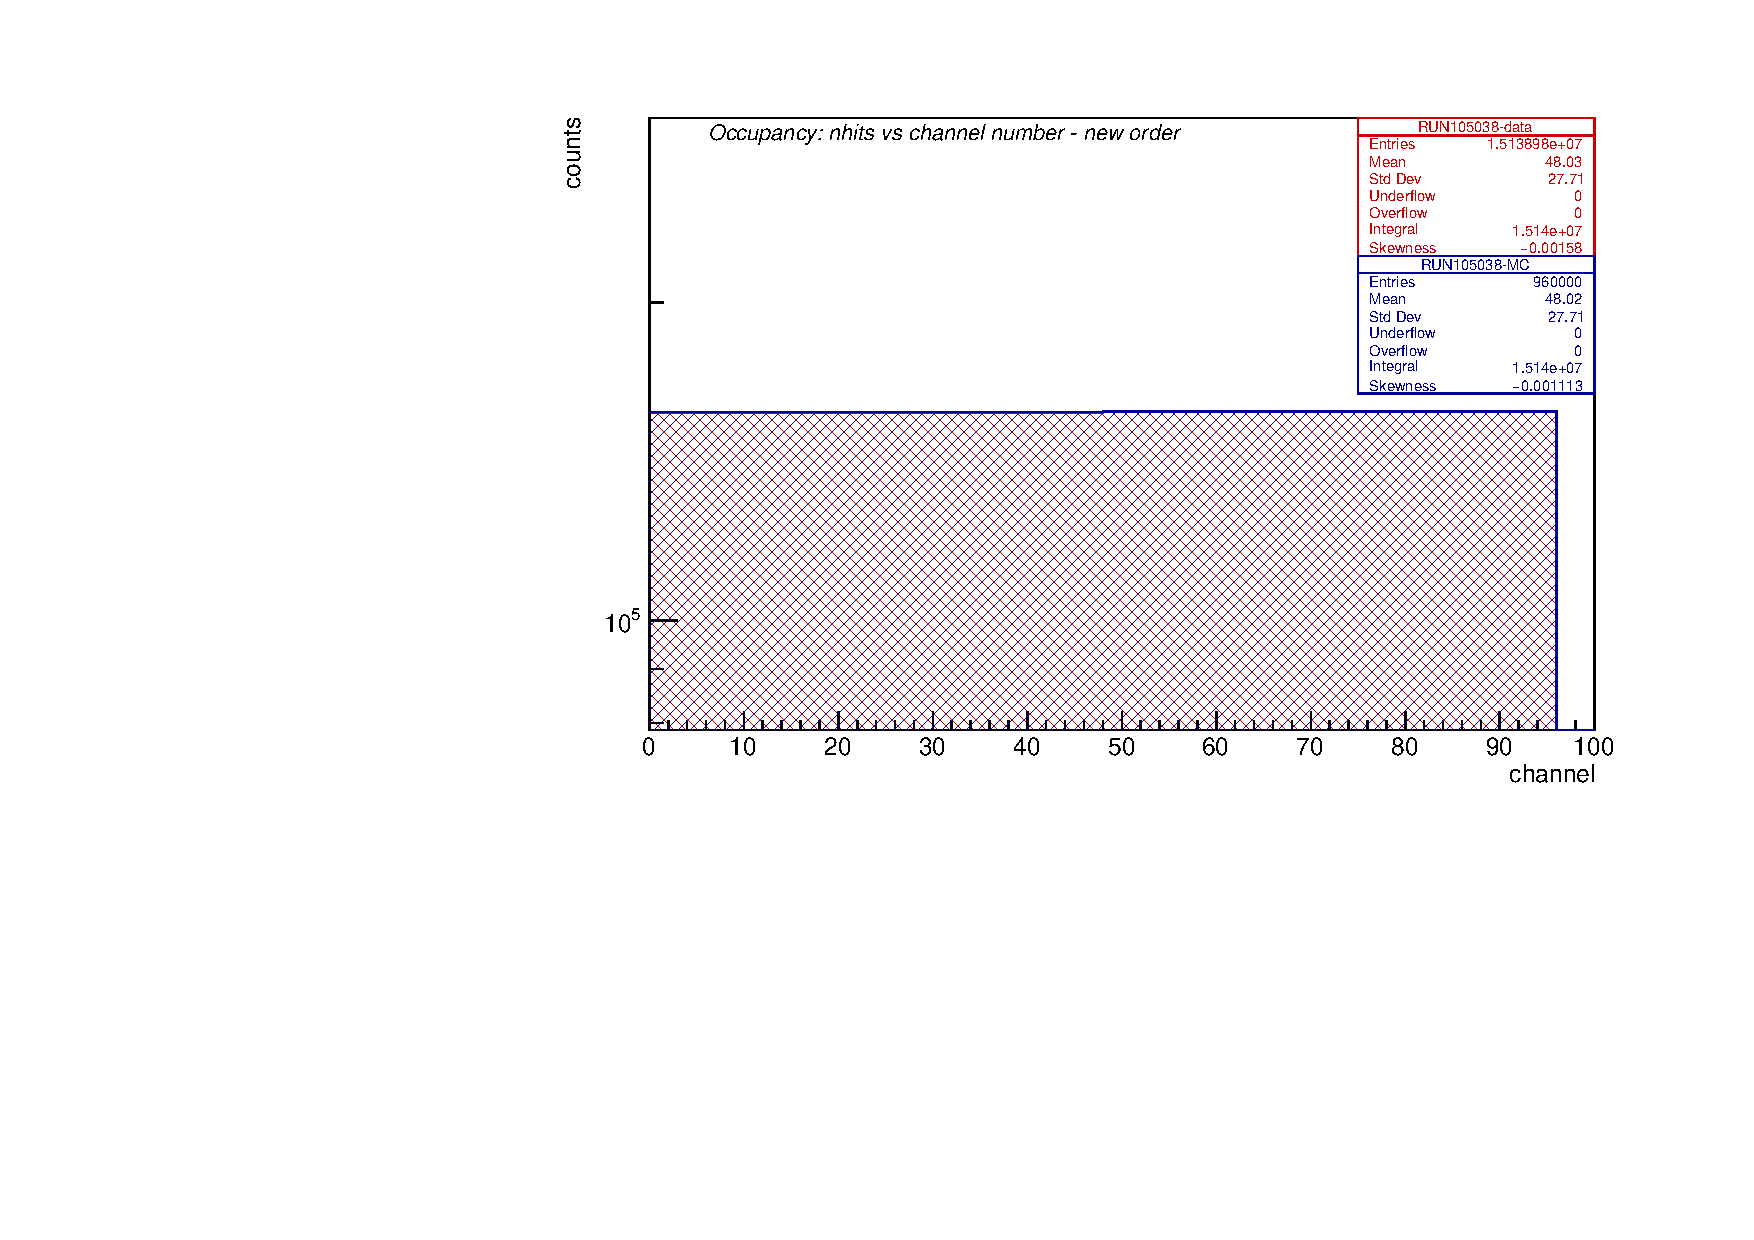
\includegraphics[width =0.8\textwidth]{figures/pdf/figure_00002_nhitsvschannel_roc_simulation_2}
\caption{Occupancy: number of hits versus channel. The ordering of channels adheres to the sequence prescribed by the Monte Carlo simulation.}
\label{fig:5}
\end{figure}
We can see a perfect adherence between data and simulation.
\subsection{Number of hits}
As conclusion we can see in Fig. \ref{fig:6}, the main aspect of non-overflow mode: the number of hits are not anymore peaked in 255 and so this reflects in the fact that the number of bytes are not always the same.
\begin{figure}[!h]
\centering
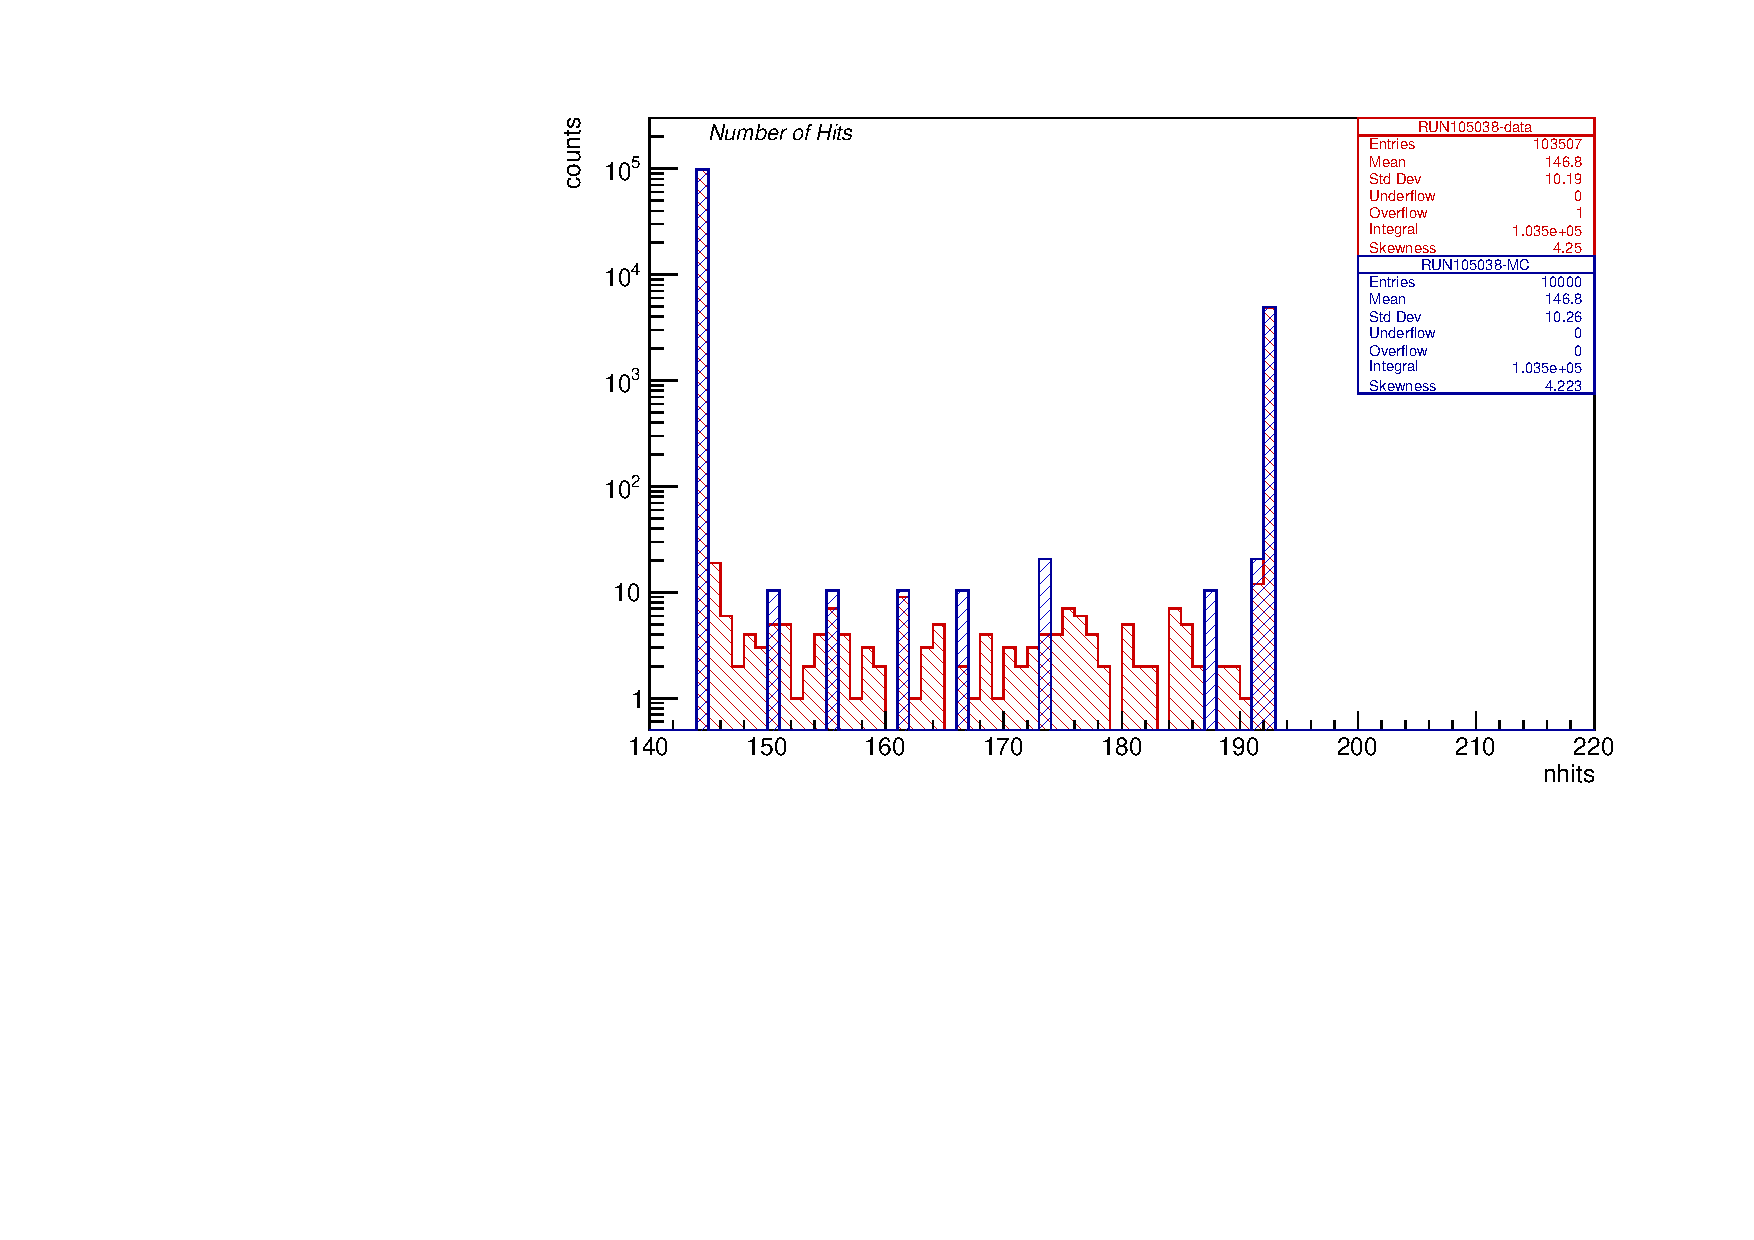
\includegraphics[width =0.8\textwidth]{figures/pdf/figure_00009_nhits_105038}
\caption{Number of hits distribution.}
\label{fig:6}
\end{figure}










%%% Local Variables:
%%% mode: latex
%%% TeX-master: t
%%% End:

% 
\section{rate}

%%%%%%%%%%%%%%%%%%%%%%%%%%%%%%%%%%%%%%%%%%%%%%%%%%%%%%%%%%%%%%%%%%%%%%%%%%%%%%
\newpage
\section{Summary}
The initial studies of the tracker readout show that the logic of the ROC and digi FPGA
firmware performs as expected. Tests of the DRAC readout in different modes show very good 
agreement with the simulation.
%%%%%%%%%%%%%%%%%%%%%%%%%%%%%%%%%%%%%%%%%%%%%%%%%%%%%%%%%%%%%%%%%%%%%%%%%%%%%%
%
%%%%%%%%%%%%%%%%%%%%%%%%%%%%%%%%%%%%%%%%%%%%%%%%%%%%%%%%%%%%%%%%%%%%%%%%%%%%%%
\newpage
\appendix\label{order}
\section{Channel readout order}
\begin{center}
\begin{tabular}{cc}
\textbf{First FPGA (CAL)}: & \\
&91,85,79,73,67,61,55,49,\\
\textit{lane 1}: &43,37,31,25,19,13,7,1,\\
&90,84,78,72,66,60,54,48,\\
& \\
&42,36,30,24,18,12,6,0,\\
\textit{lane 2}: &93,87,81,75,69,63,57,51,\\
&45,39,33,27,21,15,9,3,\\
\textbf{Second FPGA (HV)}:&\\
&\\
&38,44,5,11,17,23,29,35,\\
\textit{lane 1}:&41,92,2,8,14,20,26,32,\\
&86,80,74,68,62,56,50,47,\\
 & \\
&95,89,83,22,16,28,34,40,\\
\textit{lane 2}:&46,53,59,65,71,77,10,4,\\
&94,88,82,76,70,64,58,52\\
\end{tabular}
\end{center}   
\bibliographystyle{unsrtnat}
\bibliography{local,clfv,dio,mu2e_internal_notes}

\end{document}

